% arara: pdflatex: {synctex: yes, interaction: nonstopmode}
% arara: pdflatex: {synctex: yes, interaction: nonstopmode} until !( found('log', 'LaTeX Warning: Citation') || found('log', 'LaTeX Warning: Label') || found('log', 'LaTeX Warning: Reference') || found('log', 'There were undefined references') )

% if `LaTeX Warning: Citation' found in log, run `arara root.tex` again

%%%
 % File: /latex/big-cocluster-paper/root.tex
 % Created Date: Thursday, July 11th 2024
 % Author: Zihan
 % -----
 % Last Modified: Tuesday, 15th October 2024 4:56:30 pm
 % Modified By: the developer formerly known as Zihan at <wzh4464@gmail.com>
 % -----
 % HISTORY:
 % Date      		By   	Comments
 % ----------		------	---------------------------------------------------------
%%%

\documentclass[letterpaper, 10 pt, conference]{ieeeconf}  % Comment this line out if you need a4paper
%\documentclass[a4paper, 10pt, conference]{ieeeconf}      % Use this line for a4 paper
\IEEEoverridecommandlockouts                              % This command is only needed if 
                                                          % you want to use the \thanks command
\overrideIEEEmargins                                      % Needed to meet printer requirements.

% \usepackage{arxiv}
\usepackage{algorithm,algorithmic}
\usepackage{bm}
\usepackage{amsmath}
\let\proof\relax
\let\endproof\relax
\usepackage{amsthm}

\usepackage[utf8]{inputenc} % allow utf-8 input
\usepackage[T1]{fontenc}    % use 8-bit T1 fonts
\usepackage{hyperref}       % hyperlinks
\usepackage{url}            % simple URL typesetting
\usepackage{booktabs}       % professional-quality tables
\usepackage{amsfonts}       % blackboard math symbols
\usepackage{nicefrac}       % compact symbols for 1/2, etc.
\usepackage{microtype}      % microtypography
\usepackage{cleveref}       % smart cross-referencing
\usepackage{lipsum}         % Can be removed after putting your text content
\usepackage{graphicx}
\usepackage{multirow}       % multirow in table
% \usepackage[numeric]{natbib}
% \usepackage[backend=biber,style=ieee]{biblatex}
% \bibliography{references}  
% \DeclareFieldFormat{url}{}
% \DeclareFieldFormat{urldate}{}
\usepackage{doi}
\usepackage{threeparttable}
\usepackage{xcolor}
\usepackage{subcaption}

 
% theorems
% \usepackage{amsthm}
\newtheorem{theorem}{Theorem}
\newtheorem{lemma}{Lemma}
\newtheorem{definition}{Definition}
\newtheorem{assumption}{Assumption}

% Cref for lemma
\crefname{lemma}{lemma}{lemmas}
\Crefname{lemma}{Lemma}{Lemmas}
\crefname{assumption}{assumption}{assumptions}
\Crefname{assumption}{Assumption}{Assumptions}
\crefname{definition}{definition}{definitions}
\Crefname{definition}{Definition}{Definitions}

% set import path of input files
\makeatletter
\def\input@path{{sections/}}
\makeatother

% set image path
\graphicspath{{images/}}

\title{\LARGE \bf Scalable Co-Clustering for Large-Scale Data through Dynamic Partitioning and Hierarchical Merging}

\author{Zihan Wu$^{1}$, Zhaoke Huang$^{2}$, and Hong Yan$^{3}$, \textit{Fellow, IEEE}% <-this % stops a space
\thanks{This work is supported by Hong Kong Innovation and
Technology Commission (InnoHK Project CIMDA) and Hong
Kong Research Grants Council (Project CityU 11204821).}% <-this % stops a space
\thanks{$^{1}$Zihan Wu (Corresponding Author) is with the Department of Electrical Engineering,
        City University of Hong Kong, Hong Kong
        {\tt\small zihan.wu@my.cityu.edu.hk}}%
\thanks{$^{2}$Zhaoke Huang is with the Department of Electrical Engineering,
        City University of Hong Kong, Hong Kong
        {\tt\small Z.Huang@cityu.edu.hk}}%
\thanks{$^{3}$Hong Yan, \textit{Fellow, IEEE}, is with the Department of Electrical Engineering,
        City University of Hong Kong, Hong Kong
        {\tt\small h.yan@cityu.edu.hk}}%
}
\hypersetup{
pdftitle={Scalable Co-Clustering for Large-Scale Data through Dynamic Partitioning and Hierarchical Merging},
pdfsubject={Artificial Intelligence, Machine Learning, Data Mining},
pdfauthor={Zihan Wu, Zhaoke Huang, Hong Yan},
pdfkeywords={Co-clustering, Large-scale data, Matrix partitioning, Hierarchical merging},
}

\begin{document}
\maketitle

\thispagestyle{empty}
\pagestyle{empty}

%%%
 % File: /latex/big-cocluster-paper/sections/abstract.tex
 % Created Date: Thursday, July 11th 2024
 % Author: Zihan
 % -----
 % Last Modified: Sunday, 14th July 2024 9:43:19 pm
 % Modified By: the developer formerly known as Zihan at <wzh4464@gmail.com>
 % -----
 % HISTORY:
 % Date      		By   	Comments
 % ----------		------	---------------------------------------------------------
%%%

\begin{abstract}
Co-clustering simultaneously clusters rows and columns, revealing more fine-grained groups. However, existing co-clustering methods suffer from poor scalability and cannot handle large-scale data. This paper presents a novel and scalable co-clustering method designed to uncover intricate patterns in high-dimensional, large-scale datasets. Specifically, we first propose a large matrix partitioning algorithm that partitions a large matrix into smaller submatrices, enabling parallel co-clustering. This method employs a probabilistic model to optimize the configuration of submatrices, balancing the computational efficiency and depth of analysis.
Additionally, we propose a hierarchical co-cluster merging algorithm that efficiently identifies and merges co-clusters from these submatrices, enhancing the robustness and reliability of the process. Extensive evaluations validate the effectiveness and efficiency of our method. Experimental results demonstrate a significant reduction in computation time, with an approximate 83\% decrease for dense matrices and up to 30\% for sparse matrices.

\end{abstract}
%%%
% File: /latex/big-cocluster-paper/sections/introduction.tex
% Created Date: Thursday, July 11th 2024
% Author: Zihan
% -----
% Last Modified: Sunday, 14th July 2024 9:44:18 pm
% Modified By: the developer formerly known as Zihan at <wzh4464@gmail.com>
% -----
% HISTORY:
% Date      		By   	Comments
% ----------		------	---------------------------------------------------------
%%%

\section{Introduction}
Artificial Intelligence is a rapidly advancing technology facilitating complex data analysis, pattern recognition, and decision-making processes. Clustering, a fundamental unsupervised learning technique, groups data points based on shared features, aiding in interpreting complex data structures. However, traditional clustering algorithms \cite{zhang2023AdaptiveGraphConvolution, wu2023EffectiveClusteringStructured} treat all features of data uniformly and solely cluster either rows (samples) or columns (features),  as shown in Figure \ref{fig:cluster}. They oversimplified interpretations and overlooked critical context-specific relationships within the data, especially when dealing with large, high-dimensional datasets \cite{chen2023FastFlexibleBipartite, zhao2023MultiviewCoclusteringMultisimilarity, kumar2023CoclusteringBasedMethods}.

\textit{Co-clustering} \cite{kluger2003SpectralBiclusteringMicroarray, yan2017CoclusteringMultidimensionalBig} is a technique that groups rows (samples) and columns (features) simultaneously, as shown in Figure \ref{fig:cocluster}. It can reveal complex correlations between two different data types and is transformative in scenarios where the relationships between rows and columns are as important as the individual entities themselves. For example, in bioinformatics, co-clustering could identify gene-related patterns leading to biological insights by concurrently analyzing genes and conditions \cite{higham2007SpectralClusteringIts, kluger2003SpectralBiclusteringMicroarray, zhao2012BiclusteringAnalysisPattern}. In recommendation systems, co-clustering can simultaneously discover more fine-grained relationships between users and projects \cite{dhillon2007WeightedGraphCuts, chen2023ParallelNonNegativeMatrix}. Co-clustering extends traditional clustering methods, enhancing accuracy in pattern detection and broadening the scope of analyses.

% insert cocomparison.png here
\begin{figure}[htbp]
    \centering
    \begin{subfigure}[b]{0.22\textwidth}
        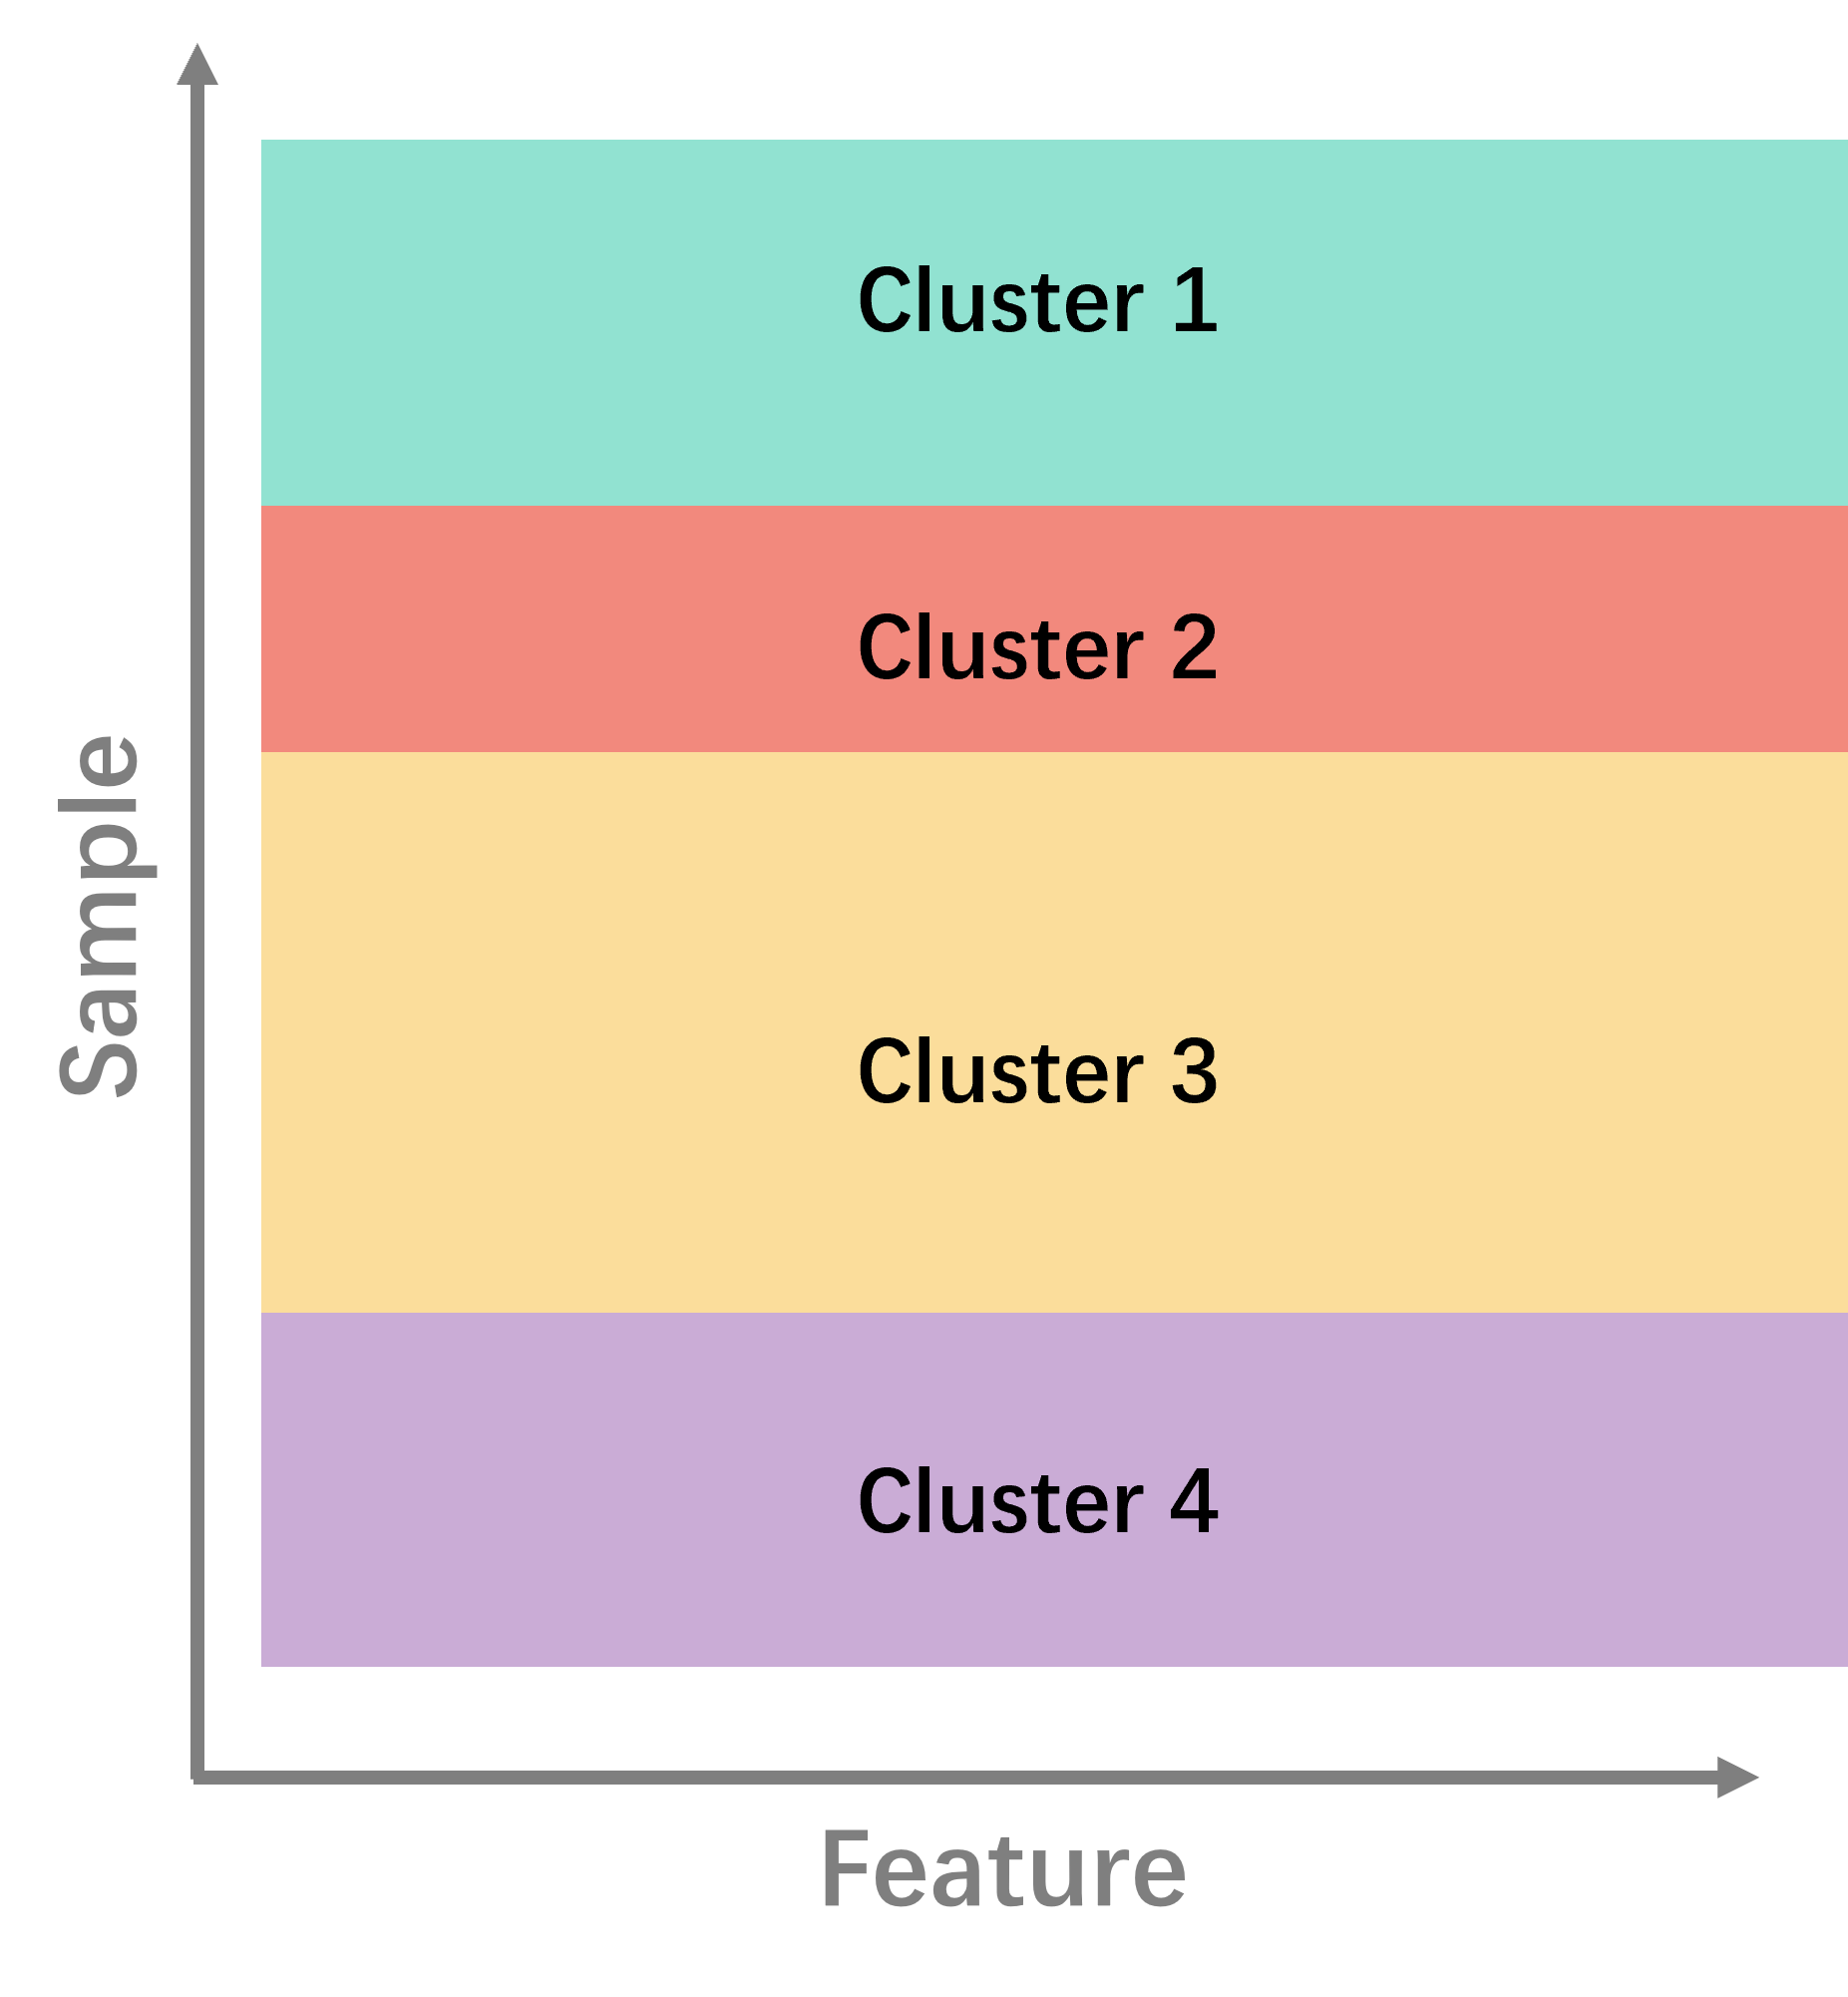
\includegraphics[width=\linewidth]{cluster.png}
        \caption{Clustering}
        \label{fig:cluster}
    \end{subfigure}
    \hfill
    \begin{subfigure}[b]{0.22\textwidth}
        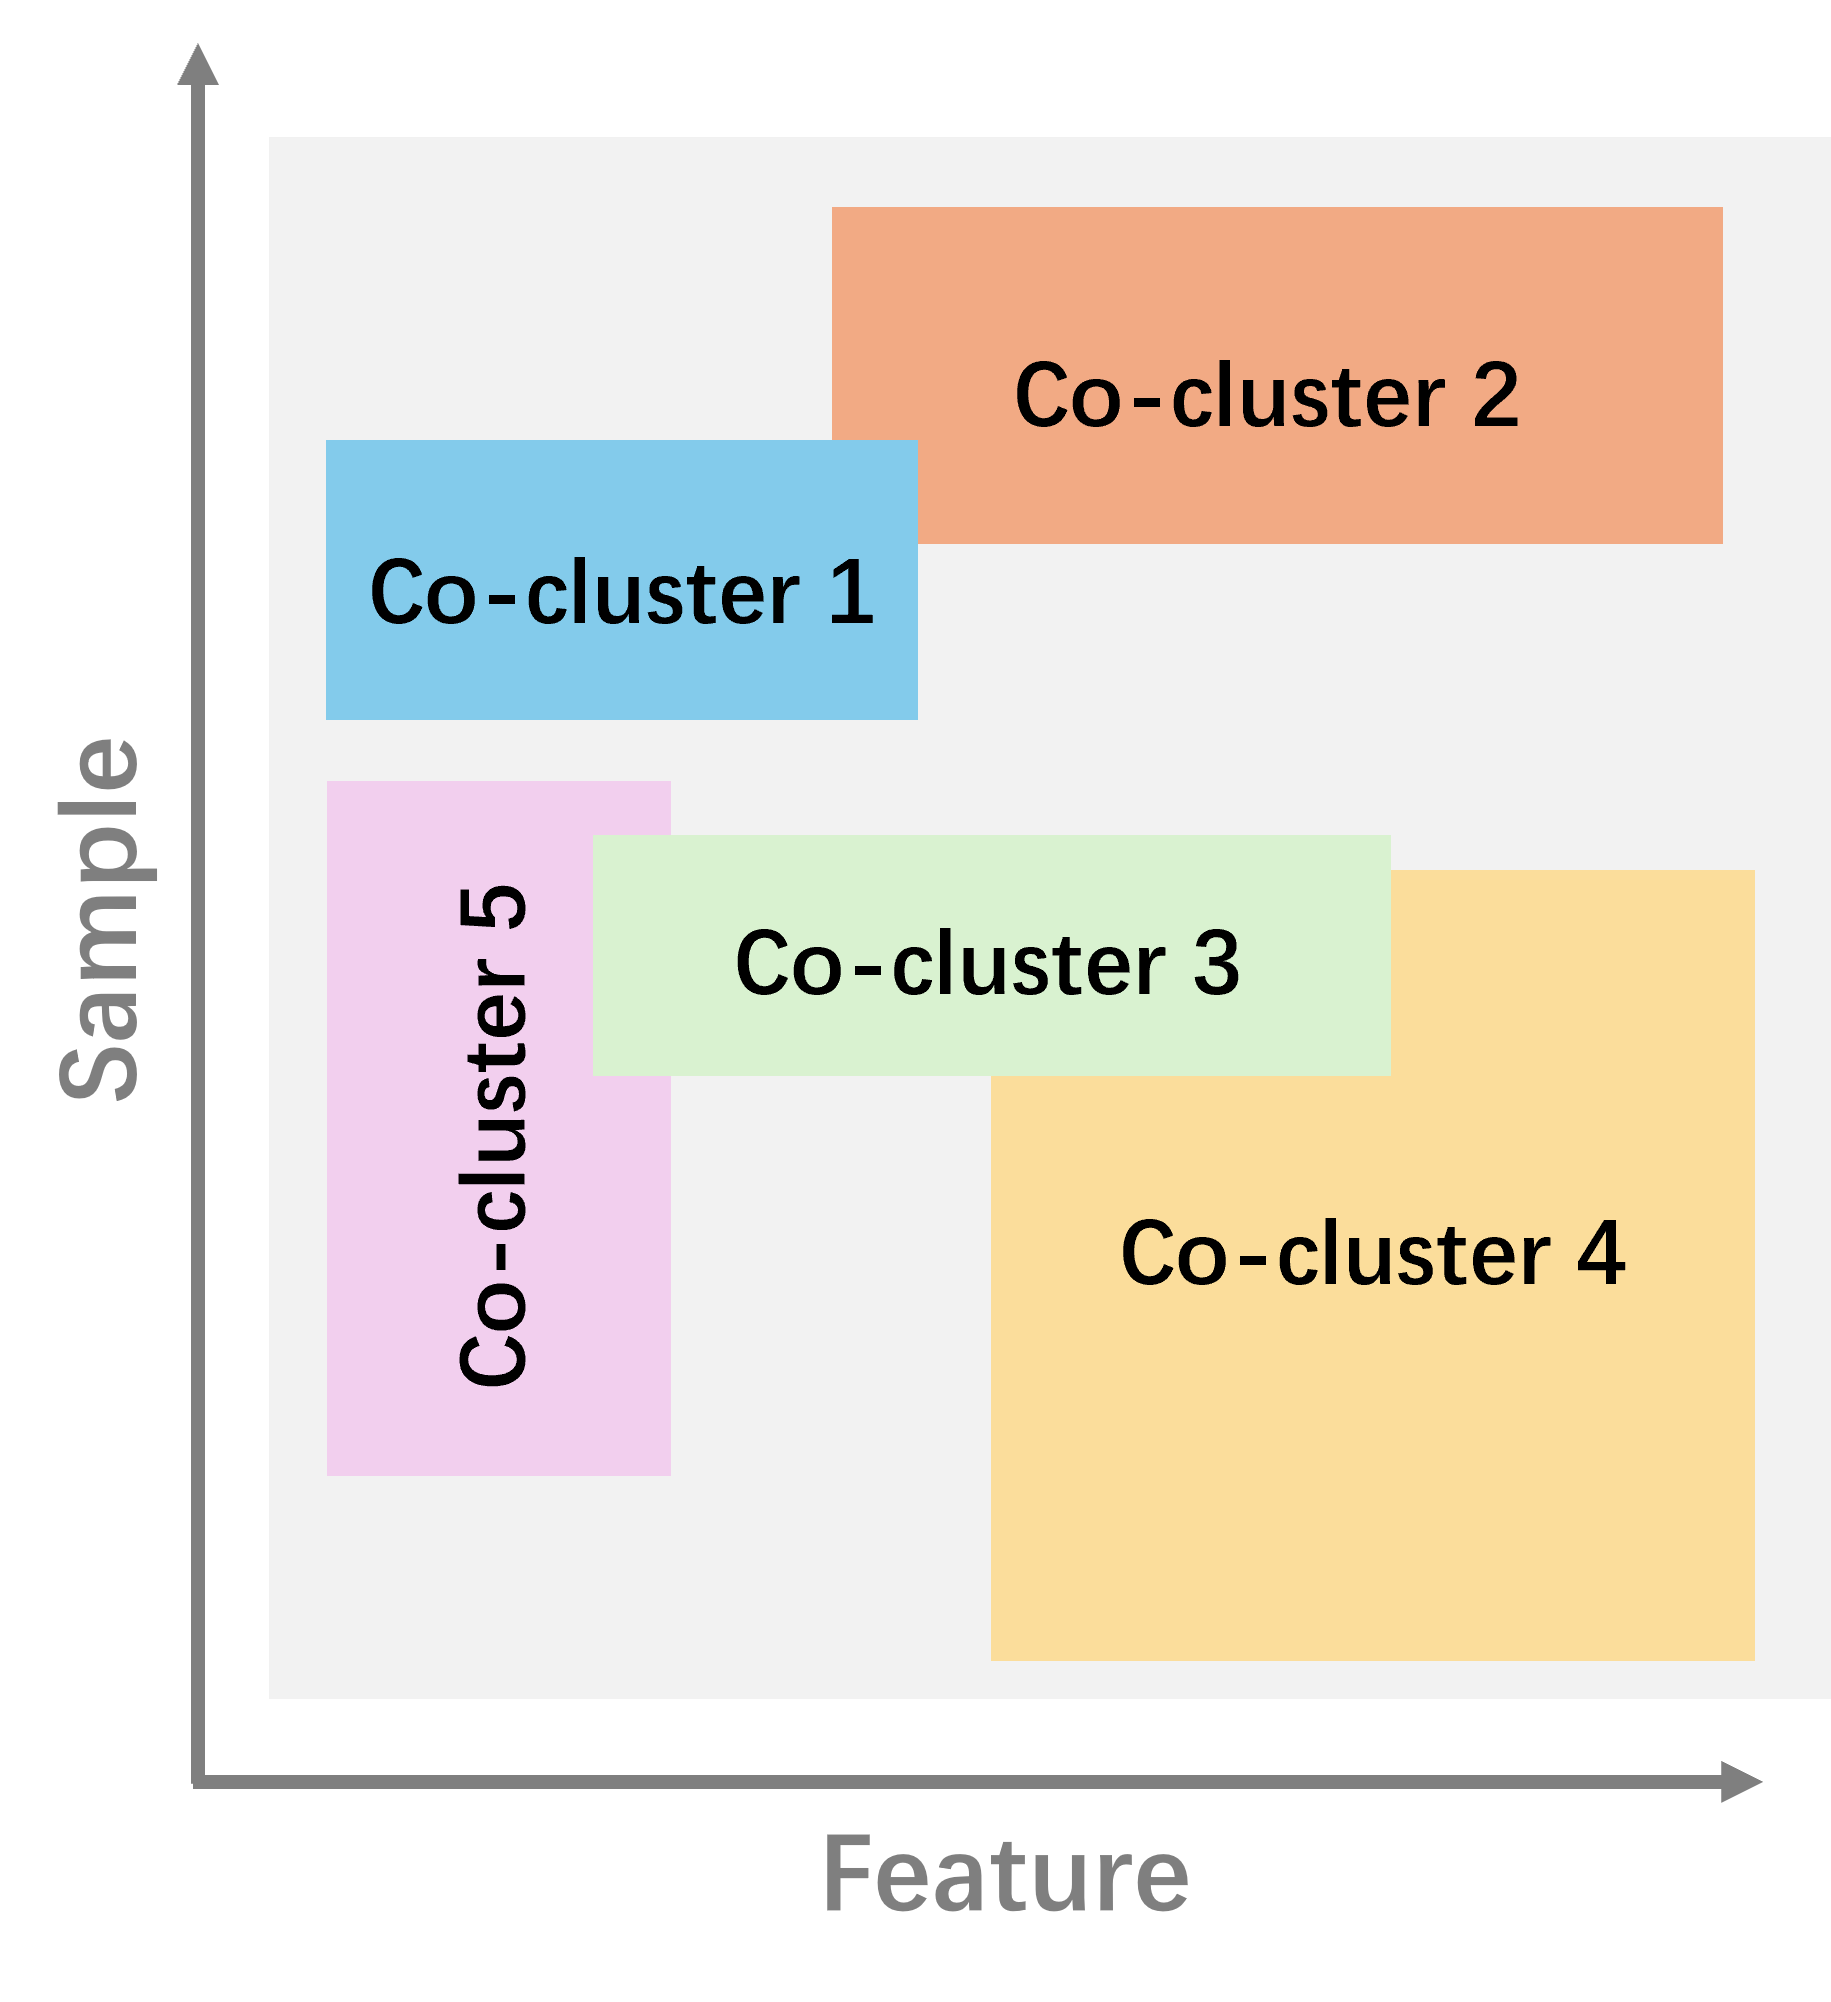
\includegraphics[width=\linewidth]{coc.png}
        \caption{Co-clustering}
        \label{fig:cocluster}
    \end{subfigure}
    \caption{An illustration of the differences between (a) Clustering and (b) Co-clustering \cite{yan2017CoclusteringMultidimensionalBig}.}
    \label{fig:cocomparison}
\end{figure}

Despite its potential, scaling co-clustering to large datasets poses significant challenges:

\begin{itemize}
    \item{\textbf{High Computational Complexity.}} Co-clustering analyzes relationships both within and across the rows and columns of a dataset simultaneously. This dual-focus analysis requires evaluating a vast number of potential relationships, particularly as the dimensions of the data increase. The complexity can grow exponentially with the size of the data because the algorithm must process every possible combination of rows and columns to identify meaningful clusters \cite{hansen2011NonparametricCoclusteringLarge}.
    \item{\textbf{Significant Communication Overhead.}} Even when methods such as data partitioning are used to handle large-scale data, each partition may independently analyze a subset of the data. However, to optimize the clustering results globally, these partitions need to exchange intermediate results frequently. This requirement is inherent to iterative optimization techniques used in co-clustering, where each iteration aims to refine the clusters based on new data insights, necessitating continuous updates across the network. Such extensive communication can become a bottleneck, significantly slowing down the overall processing speed.
    \item{\textbf{Dependency on Sparse Matrices.}} Several traditional co-clustering algorithms are designed to perform best with sparse matrices \cite{pan2008CRDFastCoclustering}. However, in many real-world applications, data matrices are often dense, meaning most elements are non-zero. Such scenarios present a significant challenge for standard co-clustering algorithms, as they must handle a larger volume of data without the computational shortcuts available with sparse matrices.
\end{itemize}

To address the inherent challenges associated with existing co-clustering methods, we propose a novel and scalable Adaptive Hierarchical Partitioning and Merging for Scalable Co-Clustering (\textbf{AHPM}) framework designed for large-scale datasets. First,  we propose a large matrix partitioning algorithm that divides the original data matrix into smaller submatrices. This partitioning facilitates parallel processing of co-clustering tasks across submatrices, significantly reducing both processing time and computational and storage demands for each processing unit. We also design a probabilistic model to determine the optimal number and configuration of these submatrices to ensure comprehensive data coverage.
Second, we develop a hierarchical co-cluster merging algorithm that iteratively combines the co-clusters from these submatrices. This process enhances the accuracy and reliability of the final co-clustering results and ensures robust and consistent clustering performance, particularly addressing issues of heterogeneity and model uncertainty.

The contributions of this paper are summarized as follows:
\begin{enumerate}
    \item \textbf{Large Matrix Partitioning Algorithm:}
          We propose a novel matrix partitioning algorithm that enables parallel co-clustering by dividing a large matrix into optimally configured submatrices. This design is supported by a probabilistic model that calculates the optimal number and order of submatrices, balancing computational efficiency with the detection of relevant co-clusters.
    \item \textbf{Hierarchical Co-cluster Merging Algorithm:}
          We design a hierarchical co-cluster merging algorithm that combines co-clusters from submatrices, ensuring the completion of the co-clustering process within a pre-fixed number of iterations. This algorithm significantly enhances the robustness and reliability of the co-clustering process, effectively addressing model uncertainty.
    \item \textbf{Experimental Valuation:}
          We evaluate the effectiveness and efficiency of our method across a wide range of scenarios with large, complex data. Experimental results show an approximate 83\% decrease for dense matrices and up to 30\% for sparse matrices.
\end{enumerate}

The rest of this paper is organized as: Section \ref{sec:related_work} reviews related works; Section \ref{sec:formula} presents the problem formulation; Section \ref{sec:method} describes our AHPM method; Section \ref{sec:experiment} reports experimental results; and Section \ref{sec:conclude} concludes the paper.

%%%
% File: /latex/big-cocluster-paper/sections/related_work.tex
% Created Date: Thursday, July 11th 2024
% Author: Zihan
% -----
% Last Modified: Sunday, 14th July 2024 9:43:56 pm
% Modified By: the developer formerly known as Zihan at <wzh4464@gmail.com>
% -----
% HISTORY:
% Date      		By   	Comments
% ----------		------	---------------------------------------------------------
%%%

\section{Related work}
\label{sec:related_work}
\subsection{Co-clustering Methods}
Co-clustering methods, broadly categorized into graph-based and matrix factorization-based approaches, have limitations in handling large datasets. Graph-based methods like Flexible Bipartite Graph Co-clustering (FBGPC) \cite{chen2023FastFlexibleBipartite} directly apply flexible bipartite graph models. Matrix factorization-based methods, such as Non-negative Matrix Tri-Factorization (NMTF) \cite{long2005CoclusteringBlockValue}, decompose data to cluster samples and features separately. Deep Co-Clustering (DeepCC) \cite{dongkuanxu2019DeepCoClustering}, which integrates deep autoencoders with Gaussian Mixture Models, also faces efficiency challenges with diverse data types and large datasets.

\subsection{Parallelizing Co-clustering}
Parallel methods are crucial for big data processing. The CoClusterD framework \cite{cheng2015CoClusterDDistributedFramework} uses Alternating Minimization Co-clustering (AMCC) in a distributed environment but struggles with guaranteed convergence. Chen \textit{et al.} \cite{chen2023ParallelNonNegativeMatrix} introduced a parallel non-negative matrix tri-factorization method to accelerate computations but still faces difficulties with very large datasets.

Our method addresses these challenges with a divide-and-conquer strategy, partitioning large matrices into smaller submatrices for parallel co-clustering, and then hierarchically merging the results. This approach significantly enhances scalability and efficiency, providing a robust solution for high-dimensional big data.

% @Author: Zihan Wu
% @Date:   2024-04-20 21:21:00
% @Last Modified by:   Zihan Wu
% @Last Modified time: 2024-04-30 23:52:00
% sectionis/method.tex

\section{Mathematical Formulation and Problem Statement}\label{sec:formula}

\subsection{Mathematical Formulation of Co-clustering}
Co-clustering groups rows and columns of a data matrix $\mathbf{A} \in \mathbb{R}^{M \times N}$, where $M$ is the number of features and $N$ is the number of samples. Each element $a_{ij}$ represents the $i$-th feature of the $j$-th sample. The goal is to partition $\mathbf{A}$ into $k$ row clusters and $d$ column clusters, creating $k \times d$ homogeneous submatrices $\mathbf{A}_{I, J}$.

When optimally reordered, $\mathbf{A}$ forms a block-diagonal structure where each block is a co-cluster with high internal similarity. Row and column labels are \( u \in \{1,\dots,k\}^M \) and \( v \in \{1,\dots,d\}^N \). Indicator matrices \( R \in \mathbb{R}^{M \times k} \) and \( C \in \mathbb{R}^{N \times d} \) assign rows and columns to clusters, ensuring unique assignments.

\subsection{Problem Statement}
This paper aims to develop a method to efficiently and accurately identify co-clusters $\mathbf{A}_{I, J}$ in large datasets. These co-clusters should exhibit uniformity, consistency, or specific patterns. Proper identification and categorization of these patterns are crucial for understanding complex data structures. Our method enhances co-clustering detection capabilities, improving efficiency and precision for large-scale data challenges.

\begin{table*}[h]
    \centering
    \begin{tabular}{c|p{10cm}}
        \hline
        \textbf{Symbol}        & \textbf{Description}                                                                                                           \\
        \hline
        $\mathbf{A}$           & Data matrix of dimensions $M \times N$, where $M$ is the number of rows (features) and $N$ is the number of columns (samples). \\
        $a_{ij}$               & Element at the $i$-th row and $j$-th column of matrix $\mathbf{A}$.                                                            \\
        $I, J$                 & Indices of rows and columns selected for co-clustering.                                                                        \\
        $\mathbf{A}_{I, J}$    & Submatrix containing the rows indexed by $I$ and columns by $J$.                                                               \\
        $R, C$                 & Indicator matrices for row and column cluster assignments.                                                                     \\
        $\phi_i, \psi_j$       & Block sizes in rows and columns, respectively.                                                                                 \\
        $s_i^{(k)}, t_j^{(k)}$ & Minimum row and column sizes of co-cluster $C_k$ in block $B_{(i,j)}$.                                                         \\
        $P(\omega_k)$          & Probability of failure to identify co-cluster $C_k$.                                                                           \\
        $T_p$                  & Number of sampling times or iterations in the probabilistic model.                                                             \\
        \hline
    \end{tabular}
    \caption{Notations used in the mathematical formulation of co-clustering}
    \label{tab:notations}
\end{table*}

\section{The Scalable Co-clustering Method}
\label{sec:method}
\subsection{Overview}

% insert workflow.png here
\begin{figure*}[htbp]
    \centering
    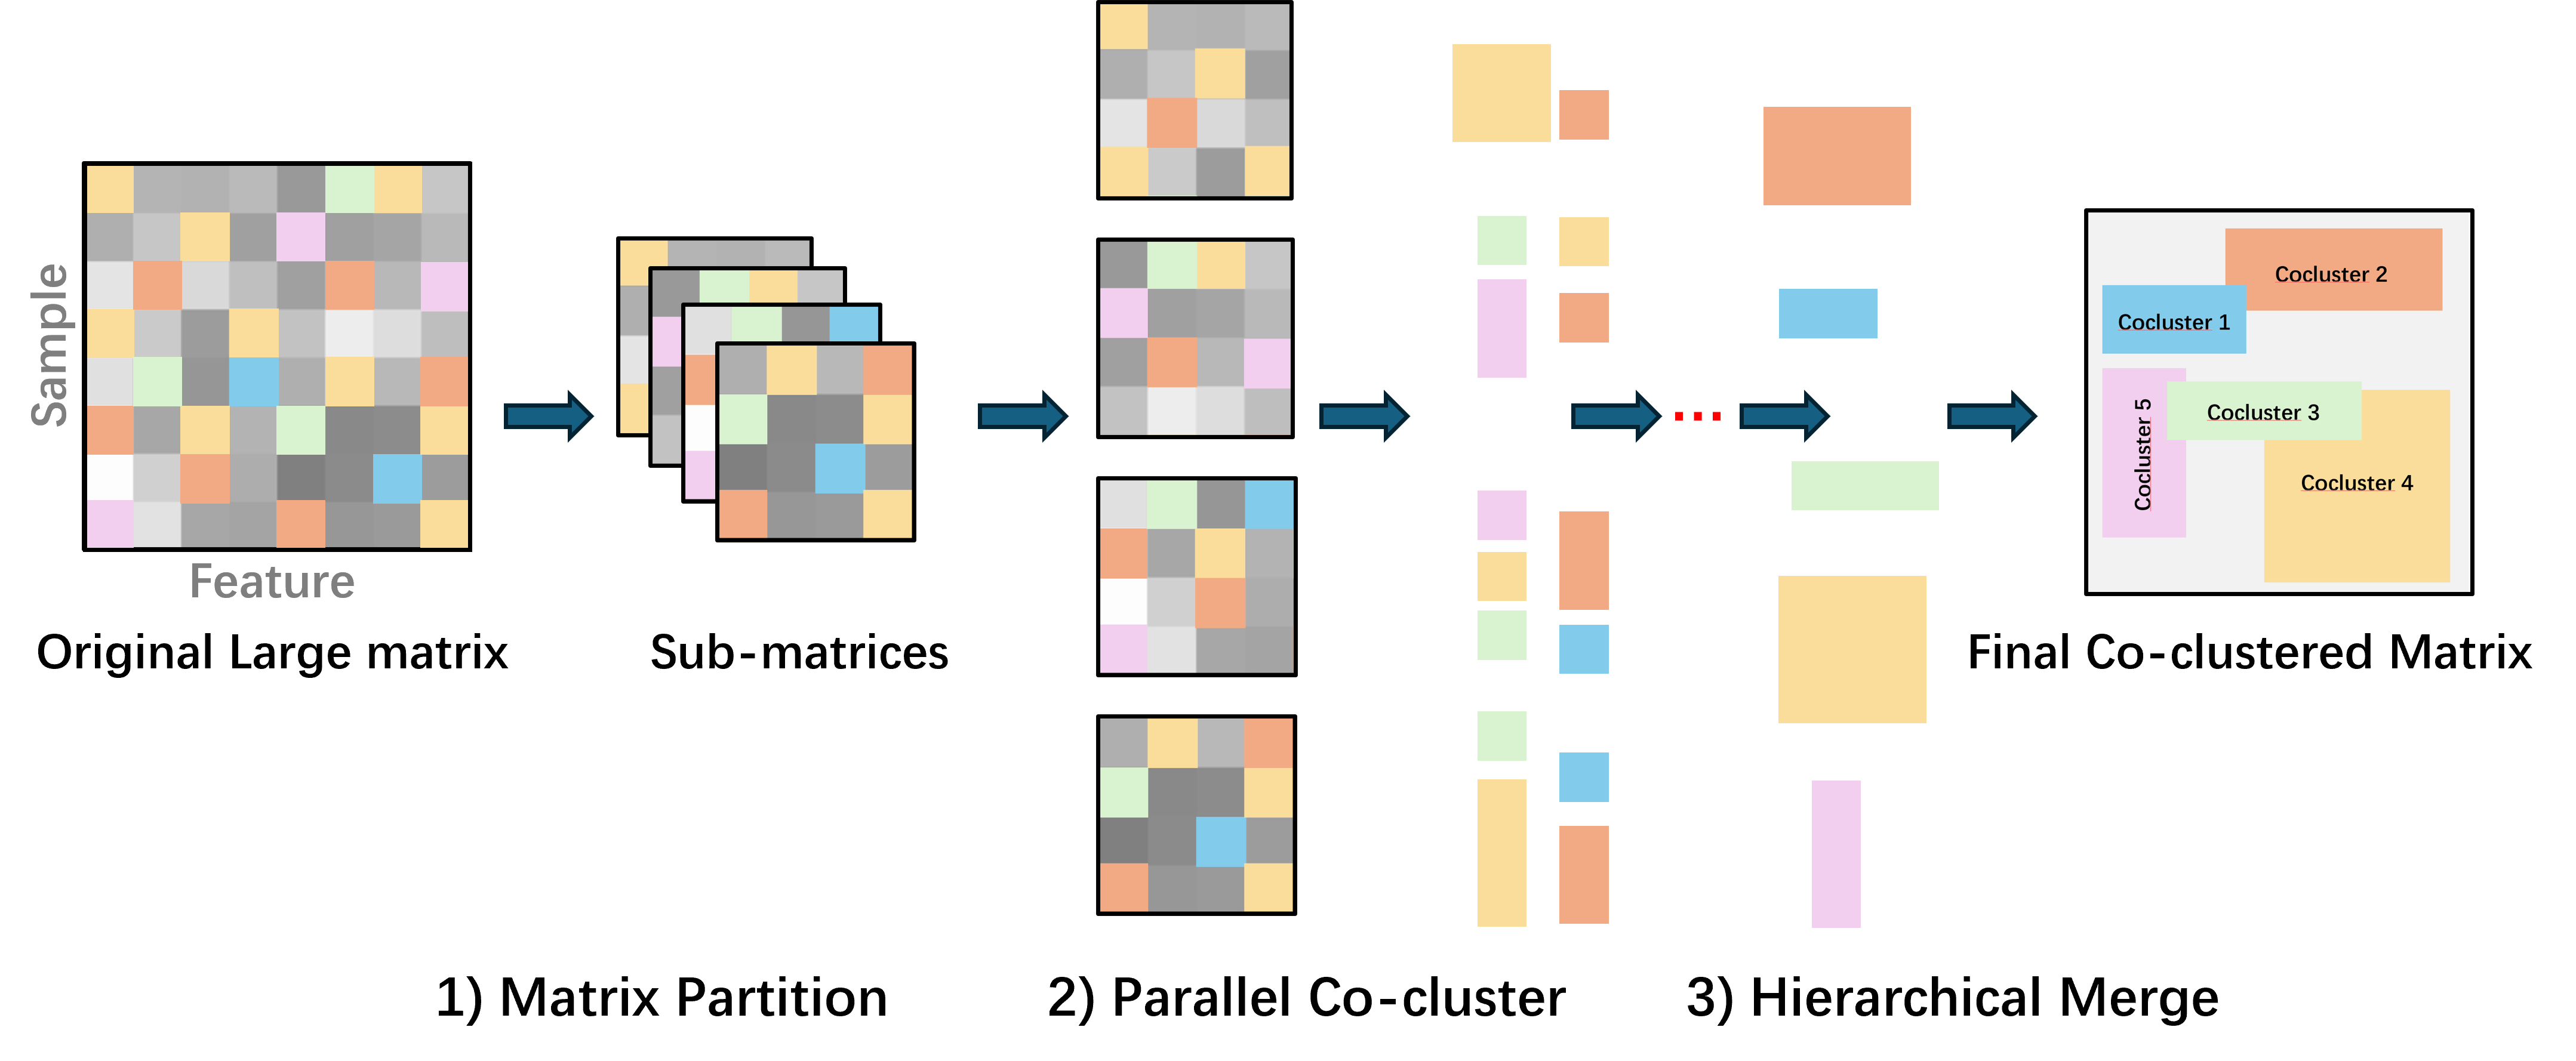
\includegraphics[width=0.8\linewidth]{workflow.png}
    \caption{Workflow of our proposed AHPM for large matrices.}
    \label{fig:workflow}
\end{figure*}
This paper presents a novel and scalable co-cluster method specifically designed for large matrices, as shown in \Cref{fig:workflow}. This method applies a probabilistic model-based optimal partitioning algorithm, which not only predicts the ideal number and sequence of partitions for maximizing computational efficiency but also ensures the effectiveness of the co-clustering process.

Our method involves partitioning large matrices into smaller, manageable submatrices. This strategic partitioning is meticulously guided by our algorithm to facilitate parallel processing. By transforming the computationally intensive task of co-clustering a large matrix into smaller, parallel tasks, our approach significantly reduces computational overhead and enhances scalability.

Following the partitioning, each submatrix undergoes a co-clustering process. This is implemented via the application of Singular Value Decomposition (SVD) and $k$-means clustering on the resulting singular vectors. This pivotal step ensures the adaptability of our method, allowing our algorithm to tailor its approach to the unique characteristics of each submatrix, thus optimizing clustering results.

Furthermore, our method integrates a novel hierarchical merging strategy that combines the co-clustering results from all submatrices. This integration provides more fine-grained insight into each submatrix and enhances the overall accuracy and reliability of the co-clustering results. Our method, validated and optimized through a comprehensive process, showed efficiency in handling large-scale datasets that were never reached before.


\subsection{Large Matrix Partitioning}
% Description of the matrix partitioning process and criteria for partitioning.
The primary challenge in co-clustering large matrices is the risk of losing co-clusters when the matrix is partitioned into smaller submatrices. To address this, we introduce an optimal partitioning algorithm underpinned by a probabilistic model. This model is meticulously designed to navigate the complexities of partitioning, ensuring that the integrity of co-clusters is maintained even as the matrix is divided. The objective of this algorithm is twofold: to determine the optimal partitioning strategy that minimizes the risk of fragmenting significant co-clusters and to define the appropriate number of repartitioning iterations needed to achieve a desired success rate of co-cluster identification.

\subsubsection{Partitioning and Repartitioning Strategy based on the Probabilistic Model}
Our probabilistic model serves as the cornerstone of the partitioning algorithm. It evaluates potential partitioning schemes based on their ability to preserve meaningful co-cluster structures within smaller submatrices. The model operates under the premise that each atom-co-cluster (the smallest identifiable co-cluster within a submatrix) can be identified with a probability $p$. This probabilistic model allows us to estimate the likelihood of successfully identifying all relevant co-clusters across the partitioned submatrices.

In the scenario where the matrix $A$ is partitioned into $m \times n$ blocks, each block has size $\phi_i \times \psi_j$, that is, $M=\sum_{i=1}^m \phi_i$ and $N=\sum_{j=1}^n \psi_j$, the joint probability of $M_{(i,j)}^{(k)}$ and $N_{(i,j)}^{(k)}$ are
\begin{equation}
    \label{eq:joint_probability}
    \begin{split}
        P(M_{(i,j)}^{(k)} & < T_m, N_{(i,j)}^{(k)} < T_n)                                                                           \\
                          & = \sum_{\alpha=1}^{T_m-1} \sum_{\beta=1}^{T_n-1} P(M_{(i,j)}^{(k)} = \alpha) P(N_{(i,j)}^{(k)} = \beta) \\
                          & \le \exp[-2 (s_i^{(k)})^2 \phi_i + -2 (t_j^{(k)})^2 \psi_j]
    \end{split}
\end{equation}
where $s_i^{(k)}$ and $t_j^{(k)}$ are the minimum row and column sizes of co-cluster $C_k$ in block $B_{(i,j)}$, the size of the co-cluster $C_k$ is $M^{(k)} \times N^{(k)}$, and $M^{(k)}$ and $N^{(k)}$ are the row and column sizes of co-cluster $C_k$, respectively.

% the size of co-cluster Ck∈RM(k)×N(k)C_k \in \mathbb{R}^{M^{(k)} \times N^{(k)}} that falls into block B(i,j)B_{(i,j)} is M(k)(i,j)×N(k)(i,j)M_{(i,j)}^{(k)} \times N_{(i,j)}^{(k)};

Thus, the probability of identifying all co-clusters is given by

\begin{equation}
    \begin{split}
        P(\omega_k) & \le \exp \left\{ -2 [\phi m (s^{(k)})^2 + \psi n (t^{(k)})^2] \right\},
    \end{split}
\end{equation}
and
\begin{equation}
    \begin{split}
        P & = 1 - P(\omega_k)^{T_p}                                                                                                       \\
          & \ge 1 - \exp \left\{ -2 T_p [\phi m (s^{(k)})^2 + \psi n (t^{(k)})^2] \right\} \label{eq:prob_of_identifying_all_co_clusters}
    \end{split}
\end{equation}
where $P(\omega_k)$ is the probability of the failure of identifying co-cluster $C_k$, $T_p$ is the number of sampling times, $\phi$ and $\psi$ are the row and column block sizes, and $s^{(k)}$ and $t^{(k)}$ are the minimum row and column sizes of co-cluster $C_k$.

\Cref{eq:prob_of_identifying_all_co_clusters} is central to our algorithm for partitioning large matrices, providing a probabilistic model to optimize our strategy and preserve co-cluster integrity. It quantifies the likelihood of identifying all relevant co-clusters within partitioned blocks, helping mitigate risks of fragmentation.

Using \eqref{eq:prob_of_identifying_all_co_clusters}, we can establish a constraint between the repartitioning time $T_r$ and the partition solution $Part$, ensuring adherence to a predetermined success rate and minimizing the risk of co-cluster fragmentation. Details of these constraints are discussed in the appendix due to space limitations.

\subsubsection{Optimization and Computational Efficiency}
Optimizing the partitioning process for computational efficiency is crucial in both academic and industrial applications. Our optimization strategy focuses on minimizing running time without compromising the integrity of co-cluster identification.

We assess various partitioning configurations to balance computational resource allocation and success rate adherence. By evaluating the impact of different schemes, we identify strategies that meet co-clustering criteria and optimize resource use.

To ensure efficiency without sacrificing quality, we introduce conditions for optimization that maintain co-cluster identification success. These conditions provide a mathematical basis for balancing computational efficiency and co-cluster identification fidelity.

The optimization must satisfy:
\begin{equation}
    \label{eq:optimization_condition}
    T_p = \text{argmin}_{T_p} \{
    1 - \exp \{ -2 T_p [\phi m (s^{(k)})^2 + n (t^{(k)})^2] \} \ge P_{\text{thresh}} \}
\end{equation}

Adhering to these conditions ensures our optimization efforts preserve the effectiveness of co-cluster discovery, making the partitioning algorithm fast, efficient, and robust across various datasets and challenges.

\subsection{Co-clustering on Small Submatrices}
% Detailed method for co-clustering within each of the submatrices.

\subsubsection{Atom-co-clustering Algorithm}
Our framework, which encompasses both partitioning and ensembling, offers remarkable flexibility, allowing it to be compatible with a wide range of atom-co-clustering methods. For the sake of making this paper comprehensive and self-contained, we provide an introduction to the atom-co-cluster method herein. The only requirement for an atom-co-clustering method to be compatible with our framework is that it must be able to identify co-clusters under a given criterion with a probability $p$, or more relaxed conditions, has a lower bound estimate of the probability of identifying co-clusters equipped with a validation mechanism.

\subsubsection{Graph-based Spectral Co-clustering Algorithm}
Spectral co-clustering (SCC) is widely used for high-dimensional data due to its effectiveness in partitioning data into clusters based on graph Laplacian eigenvectors \cite{vonluxburg2007TutorialSpectralClustering}. SCC constructs a bipartite graph $G=(U,V,E)$ from the data matrix $A$, where $U$ and $V$ represent rows and columns, respectively, and $E$ are weighted edges indicating relationships.

The Laplacian matrix $L = D - W$ is computed, where $D$ is the degree matrix, and $W$ is the weighted adjacency matrix. Eigenvectors of the smallest positive eigenvalues of $L$ are used to partition the graph. The normalized matrix $A_n = D^{-1/2} A D^{-1/2}$ is factorized using singular value decomposition (SVD), and the resulting singular vectors are used for clustering.

For co-clustering, we apply $k$-means to the rows of the matrix formed by stacking the left and right singular vectors of $A_n$. This method effectively identifies clusters in high-dimensional data, making it suitable for our framework \cite{dhillon2001CoclusteringDocumentsWords}.

\begin{algorithm}[ht]
    \caption{Optimal Matrix Partition and Hierarchical Co-cluster Merging Method}\label{alg:method}
    \begin{algorithmic}[1]
        \REQUIRE{Data matrix $A \in \mathbb{R}^{M \times N}$, Co-cluster set $C = \{C_k\}_{k=1}^K$, Block sizes $\{\phi_i\}_{i=1}^m$, $\{\psi_j\}_{j=1}^n$, Thresholds $T_m$, $T_n$, Sampling times $T_p$, Probability threshold $P_\text{thresh}$;}
        \ENSURE{Co-clustered result $\mathcal{C}$;}
        \STATE Initialize block set $B = \{B_{(i,j)}\}_{i=1}^m,_{j=1}^n$ on $\phi_i$ and $\psi_j$
        \STATE Calculate $s^{(k)}$ and $t^{(k)}$ for each co-cluster $C_k$
        \FOR{$k=1$ to $K$}
        \STATE Calculate $P(\omega_k)$ for co-cluster $C_k$
        \IF{$P(\omega_k) < P_{thresh}$}
        \STATE Partition matrix $A$ into blocks $B$ and perform co-clustering
        \STATE Aggregate co-clustered results from each block
        \ENDIF
        \ENDFOR
        \RETURN Aggregated co-clustered result $\mathcal{C}$
    \end{algorithmic}
\end{algorithm}

\begin{table*}[!htbp]
    \centering
    \caption{Comparison of Running Times (in seconds) for Various Co-clustering Methods on Selected Datasets.}
    \label{tab:running-time}
    \begin{tabular}{@{} l cccc @{}}
        \toprule
        Dataset     & SCC \cite{dhillon2001CoclusteringDocumentsWords} & PNMTF \cite{chen2023ParallelNonNegativeMatrix} & \textbf{AHPM-SCC} & \textbf{AHPM-PNMTF} \\
        \midrule
        Amazon 1000 & 64545.2                                          & 303.7                                          & 112.5             & 242.8               \\
        CLASSIC4    & *                                                & 17,810                                         & 22,894            & 3,028               \\
        RCV1-Large  & *                                                & 277,092                                        & *                 & 208,048             \\
        % ... more rows here
        \bottomrule
    \end{tabular}
    \begin{tablenotes}
        \small
        \item Notes: * indicates that the method cannot process the dataset because the dataset size exceeds the processing limit.
    \end{tablenotes}
\end{table*}

\begin{table*}[!htbp]
    \centering
    \caption{NMIs and ARIs Scores for Various Co-clustering Methods on Selected Datasets.}
    \label{tab:evaluation-metrics}
    \begin{tabular}{@{} l c cccc @{}}
        \toprule
        \multirow{2}{*}{Dataset}     & \multirow{2}{*}{Metric} & \multicolumn{4}{c}{Compared Methods}                                                                                                        \\
        \cmidrule{3-6}
                                     &                         & SCC \cite{dhillon2001CoclusteringDocumentsWords} & PNMTF \cite{chen2023ParallelNonNegativeMatrix} & \textbf{AHPM-SCC} & \textbf{AHPM-PNMTF} \\
        \midrule
        \multirow{2}{*}{Amazon 1000} & NMI                     & 0.9223                                           & 0.6894                                         & 0.8650            & 0.6609              \\
                                     & ARI                     & 0.7713                                           & 0.6188                                         & 0.7763            & 0.6057              \\
        \multirow{2}{*}{CLASSIC4}    & NMI                     & *                                                & 0.5944                                         & 0.7676            & 0.6073              \\
                                     & ARI                     & *                                                & 0.4523                                         & 0.5845            & 0.4469              \\
        \multirow{2}{*}{RCV1-Large}  & NMI                     & *                                                & 0.6519                                         & 0.8349            & 0.6348              \\
                                     & ARI                     & *                                                & 0.5383                                         & 0.7576            & 0.5298              \\
        % ... more rows here
        \bottomrule
    \end{tabular}
    \begin{tablenotes}
        \small
        \item Notes: * indicates that the method cannot process the dataset because the dataset size exceeds the processing limit.
    \end{tablenotes}
\end{table*}

\subsection{Hierarchical Co-cluster Merging}
% Explanation of how co-clustered results from submatrices are aggregated.

With the co-clustering results from each submatrix in hand, the next step is to merge these results to form the final co-clustered output. This merging process employs a hierarchical strategy that starts with the most closely related clusters, gradually integrating broader groups to maintain consistency and reduce redundancy. Throughout this process, the algorithm assesses and recalibrates the similarity thresholds necessary to ensure clusters are combined appropriately, thus accommodating the diverse nature of the data. By iteratively refining the merging criteria, the framework can adaptively reconcile differences among submatrix clusters, resulting in a robust and coherent final clustering solution that reflects the inherent structure of the entire dataset. This approach not only preserves the detailed information within each subcluster but also enhances the overall clustering accuracy and reliability.

\subsection{Algorithmic Description}
% Step-by-step algorithmic description of the process in pseudocode.
Our proposed  Optimal Matrix Partition and Hierarchical Co-cluster Merging Method is outlined in Algorithm \ref{alg:method}. The algorithm
is an advanced algorithm designed for efficient co-clustering of large data matrices. The algorithm begins by initializing a block set based on predetermined block sizes. For each co-cluster in the given set, the algorithm calculates specific values $s^{(k)}$ and $t^{(k)}$, which are then used to determine the probability $P(\omega_k)$ of each co-cluster. If this probability falls below a predefined threshold $P_{\text{thresh}}$, the algorithm partitions the data matrix $A$ into blocks $B$ and performs co-clustering on these blocks. This step is crucial for managing large datasets by breaking them down into smaller, more manageable units. After co-clustering, the results from each block are aggregated to form the final co-clustered result $\mathcal{C}$. The algorithm's design allows for a flexible and efficient approach to co-clustering, particularly suited to datasets with high dimensionality and complexity.

%%%
% File: /latex/big-cocluster-paper/sections/experiment.tex
% Created Date: Thursday, July 11th 2024
% Author: Zihan
% -----
% Last Modified: Sunday, 14th July 2024 9:43:45 pm
% Modified By: the developer formerly known as Zihan at <wzh4464@gmail.com>
% -----
% HISTORY:
% Date      		By   	Comments
% ----------		------	---------------------------------------------------------
%%%

\section{Experimental Evaluation}
\label{sec:experiment}
\subsection{Experiment Setup}

\textbf{Datasets.}
The experiments were conducted using three distinct datasets to demonstrate the versatility and robustness of our method:

\begin{itemize}
    \item Amazon 1000 \cite{ni2019justifying}: Comprising 1000 Amazon reviews; each represented as a 1000-dimensional vector, this dataset is designed to mimic customer behavior analysis.
    \item CLASSIC4 \cite{reddy2021weclustering}: Containing 18000 documents from 20 newsgroups; each document is represented as a 1000-dimensional vector, this dataset is suitable for text analysis and topic discovery.
    \item RCV1-Large \cite{lewis2004rcv1}: A larger dataset used to test the scalability of our method, it includes a vast array of document vectors for high-dimensional data analysis.
\end{itemize}

\textbf{Implementation details.}
All experiments were performed on a computing cluster with the following specifications: Intel Xeon E5-2670 v3 @ 2.30GHz processors, 128GB RAM, and Ubuntu 20.04 LTS operating system. The algorithms were implemented in Rust and compiled with the latest stable version of the Rust compiler.

\textbf{Compared Methods.}
The experiments followed the procedure outlined in Algorithm \ref{alg:method}. The proposed method was compared with the following state-of-the-art co-clustering methods:

\begin{itemize}
    \item Spectral Co-Clustering (SCC) \cite{dhillon2001CoclusteringDocumentsWords}
    \item Parallel Non-negative Matrix Tri-Factorization (PNMTF)\cite{chen2023ParallelNonNegativeMatrix}
    \item Deep Co-Clustering (DeepCC) \cite{dongkuanxu2019DeepCoClustering}
\end{itemize}

Notably, 1) PNMTF is one of the most efficient co-clustering algorithms in the state-of-art. 2) All our experiments show that DeepCC cannot process all selected datasets due to the dataset size exceeds DeepCC processing limit.

\textbf{Our Methods.} Our proposed scalable co-cluster method is applied along with the SCC and PNMTF to demonstrate the enhanced performance and capability of handling large datasets:
\begin{itemize}
    \item Adaptive Hierarchical Partitioning and Merging for Scalable Co-Clustering with Spectral Co-Clustering (AHPM-SCC)
    \item Adaptive Hierarchical Partitioning and Merging for Scalable Co-Clustering with Parallel Non-negative Matrix Tri-Factorization (AHPM-PNMTF)
\end{itemize}

\textbf{Evaluation Metrics.}
The effectiveness of the co-clustering was measured using two widely accepted metrics:

\begin{itemize}
    \item Normalized Mutual Information (NMI): Quantifies the mutual information between the co-clusters obtained and the ground truth, normalized to [0, 1] range, where 1 indicates perfect overlap.
    \item Adjusted Rand Index (ARI): Adjusts the Rand Index for chance, providing a measure of the agreement between two clusters, with values ranging from $-1$ (complete disagreement) to 1 (perfect agreement).
\end{itemize}

\subsection{Results}
The experimental results are presented in Tables \ref{tab:running-time} and \ref{tab:evaluation-metrics}, comparing our methods, AHPM-SCC and AHPM-PNMTF, with traditional methods SCC and PNMTF.

\subsubsection{Handling Large-scale Datasets} The results highlight the limitations of traditional methods like SCC and DeepCC in processing large datasets, as shown by their inability to handle certain datasets (denoted by "*"). This underscores the scalability challenges in existing co-clustering methods.

\subsubsection{Improved Performance} Our methods successfully processed all datasets and significantly outperformed traditional methods in efficiency. For example, the running time for the Amazon 1000 dataset was reduced from 64545.2 seconds (SCC) to 112.5 seconds (AHPM-SCC), demonstrating a substantial increase in speed.

\subsubsection{Quantitative Metrics} As shown in Table \ref{tab:evaluation-metrics}, our methods also improved accuracy and robustness. For instance, in the CLASSIC4 dataset, AHPM-SCC achieved an NMI of 0.7676 and an ARI of 0.5845, outperforming PNMTF.

These results validate our scalable co-clustering method as more efficient and capable of handling diverse, large-scale datasets without compromising co-cluster identification quality. The adaptability and parallel processing capabilities of our method demonstrate its potential for various applications, including text and biomedical data analysis and financial pattern recognition.

%%%
% File: /latex/big-cocluster-paper/sections/conclusion.tex
% Created Date: Thursday, July 11th 2024
% Author: Zihan
% -----
% Last Modified: Sunday, 14th July 2024 9:43:36 pm
% Modified By: the developer formerly known as Zihan at <wzh4464@gmail.com>
% -----
% HISTORY:
% Date      		By   	Comments
% ----------		------	---------------------------------------------------------
%%%

\section{Conclusion}
\label{sec:conclude}
This paper introduces a novel, scalable co-clustering method for large matrices, addressing the computational challenges of high-dimensional data analysis. Our method first partitions large matrices into smaller, parallel-processed submatrices, significantly reducing processing time. Next, a hierarchical co-cluster merging algorithm integrates the submatrix results, ensuring accurate and consistent final co-clustering. Extensive evaluations demonstrate that our method outperforms existing solutions in handling large-scale datasets, proving its effectiveness, efficiency, and scalability.

% %%%
% File: /latex/big-cocluster-paper/sections/appendix.tex
% Created Date: Tuesday, January 23rd 2024
% Author: Zihan
% -----
% Last Modified: Wednesday, 27th March 2024 10:40:18 pm
% Modified By: the developer formerly known as Zihan at <wzh4464@gmail.com>
% -----
% HISTORY:
% Date      		By   	Comments
% ----------		------	---------------------------------------------------------
%%%

% \newpage
\appendix

\begin{theorem}
    \label{thm:probability_co_cluster_detection}
    If the matrix $\mathbf{A}$ is partitioned into $m \times n$ blocks, each with sizes $\phi_i \times \psi_j$, and the probability of failing to detect co-cluster $\mathbf{C}_k$ in any block is $P(\omega_k)$, then
    \begin{equation}
        \begin{split}
            P(\omega_k) & \le \exp \left\{ -2 [\phi m (s^{(k)})^2 + \psi n (t^{(k)})^2] \right\}
        \end{split}
    \end{equation}
    Given $T_p$ times of random sampling, the probability of detecting the co-cluster $C_k$ is
    \begin{equation}
        \begin{split}
            P & = 1 - P(\omega_k)^{T_p}                                                        \\
              & \ge 1 - \exp \left\{ -2 T_p [\phi m (s^{(k)})^2 + \psi n (t^{(k)})^2] \right\}
        \end{split}
    \end{equation}

\end{theorem}

\begin{proof}
    Consider co-cluster $C_k$,
    % P(M_{(i,j)}^{(k)} = i)
    \begin{equation}
        \begin{split}
            P(M_{(i,j)}^{(k)} = \alpha) & = \frac{\binom{M^{(k)}}{\alpha} \binom{M-M^{(k)}}{\phi_i-\alpha}}{\binom{M}{\phi_i}} \\
            % p[x_] := Binomial[Mk, a] * Binomial[M-Mk, P-a] / Binomial[M, P]
            P(N_{(i,j)}^{(k)} = \beta)  & = \frac{\binom{N^{(k)}}{\beta} \binom{N-N^{(k)}}{\psi_j-\beta}}{\binom{N}{\psi_j}}
            % q[y_] := Binomial[Nk, b] * Binomial[N-Nk, Q-b] / Binomial[N, Q]
        \end{split}
    \end{equation}
    The tail probability of $M_{(i,j)}^{(k)}$ and $N_{(i,j)}^{(k)}$ are
    \begin{equation}
        \begin{split}
            P(M_{(i,j)}^{(k)} < T_m) & = \sum_{\alpha=1}^{T_m-1} P(M_{(i,j)}^{(k)} = \alpha) \\
                                     & \le \exp(-2 (s_i^{(k)})^2 \phi_i)
        \end{split}
    \end{equation}
    where $s_i^{(k)} = \cfrac{M^{(k)}}{M}-\cfrac{T_m-1}{\phi_i}$, and
    \begin{equation}
        \begin{split}
            % &\le \sum_{\alpha=1}^{T_m-1} \frac{\binom{M^{(k)}}{\alpha} \binom{M-M^{(k)}}{\phi_i-\alpha}}{\binom{M}{\phi_i}} \\
            P(N_{(i,j)}^{(k)} < T_n) & = \sum_{\beta=1}^{T_n-1} P(N_{(i,j)}^{(k)} = \beta) \\
                                     & \le \exp (-2 (t_j^{(k)})^2 \psi_j)
        \end{split}
    \end{equation}
    where $t_j^{(k)} = \cfrac{N^{(k)}}{N}-\cfrac{T_n-1}{\psi_j}$.

    The joint probability of $M_{(i,j)}^{(k)}$ and $N_{(i,j)}^{(k)}$ are
    \begin{equation}
        \begin{split}
            P & (M_{(i,j)}^{(k)} < T_m, N_{(i,j)}^{(k)} < T_n)              \\ & = \sum_{\alpha=1}^{T_m-1} \sum_{\beta=1}^{T_n-1} P(M_{(i,j)}^{(k)} = \alpha) P(N_{(i,j)}^{(k)} = \beta) \\
            % pq[x_, y_] := Sum[p[a] * q[b], {a, 1, x-1}, {b, 1, y-1}]
              & \le \exp[-2 (s_i^{(k)})^2 \phi_i + -2 (t_j^{(k)})^2 \psi_j]
        \end{split}
    \end{equation}
    If $\phi_i = p$ and $\psi_j = q$ for all $i$ and $j$, then

    Suppose event $\omega_k$ is that co-cluster $C_k$ can't be find in any block $B_{(i,j)}$, then
    \begin{equation}
        \begin{split}
            P(\omega_k) & = \prod_{i=1}^m \prod_{j=1}^n P(M_{(i,j)}^{(k)} < T_m, N_{(i,j)}^{(k)} < T_n)                          \\
                        & \le \prod_{i=1}^m \prod_{j=1}^n \exp\{-2 \left[ (s_i^{(k)})^2 \phi_i + (t_j^{(k)})^2 \psi_j \right] \} \\
                        & = \exp\{-2 \sum_{i=1}^m \sum_{j=1}^n \left[ (s_i^{(k)})^2 \phi_i + (t_j^{(k)})^2 \psi_j \right] \}     \\
        \end{split}
    \end{equation}

    If $\phi_i = \phi$ and $\psi_j = \psi$ for all $i$ and $j$, then
    \begin{equation}
        \begin{split}
            s_i^{(k)} & = s^{(k)} = \frac{M^{(k)}}{M}-\frac{T_m-1}{\phi} \\
            t_j^{(k)} & = t^{(k)} = \frac{N^{(k)}}{N}-\frac{T_n-1}{\psi}
        \end{split}
    \end{equation}

    \begin{equation}
        \begin{split}
            P(\omega_k) & \le \exp \left\{ -2 [\phi m (s^{(k)})^2 + \psi n (t^{(k)})^2] \right\} \\
        \end{split}
    \end{equation}


    And if we do $T_p$ times of random sampling, the Probability of detecting the co-cluster is
    \begin{equation}
        \begin{split}
            P & = 1 - P(\omega_k)^{T_p}                                                        \\
              & \ge 1 - \exp \left\{ -2 T_p [\phi m (s^{(k)})^2 + \psi n (t^{(k)})^2] \right\} \\
        \end{split}
    \end{equation}
    according to which, we can set $m, n, \phi, \psi, T_m, T_n$ and $T_p$ to ensure the probability of detecting the co-cluster is larger than a given threshold.
\end{proof}

% \section*{Acknowledgment}
% This work is supported by Hong Kong Innovation and Technology
% Commission (InnoHK Project CIMDA) and Hong Kong Research Grants
% Council (Project CityU 11204821).

% \begin{table}[b]
% 	\caption{Sample table title}
% 	\centering
% 	\begin{tabular}{lll}
% 		\toprule
% 		\multicolumn{2}{c}{Part}                   \\
% 		\cmidrule(r){1-2}
% 		Name     & Description     & Size ($\mu$m) \\
% 		\midrule
% 		Dendrite & Input terminal  & $\sim$100     \\
% 		Axon     & Output terminal & $\sim$10      \\
% 		Soma     & Cell body       & up to $10^6$  \\
% 		\bottomrule
% 	\end{tabular}
% 	\label{tab:table}
% \end{table}

% Generated by IEEEtran.bst, version: 1.14 (2015/08/26)
\begin{thebibliography}{10}
        \providecommand{\url}[1]{#1}
        \csname url@samestyle\endcsname
        \providecommand{\newblock}{\relax}
        \providecommand{\bibinfo}[2]{#2}
        \providecommand{\BIBentrySTDinterwordspacing}{\spaceskip=0pt\relax}
        \providecommand{\BIBentryALTinterwordstretchfactor}{4}
        \providecommand{\BIBentryALTinterwordspacing}{\spaceskip=\fontdimen2\font plus
                \BIBentryALTinterwordstretchfactor\fontdimen3\font minus
                \fontdimen4\font\relax}
        \providecommand{\BIBforeignlanguage}[2]{{%
                                \expandafter\ifx\csname l@#1\endcsname\relax
                                        \typeout{** WARNING: IEEEtran.bst: No hyphenation pattern has been}%
                                        \typeout{** loaded for the language `#1'. Using the pattern for}%
                                        \typeout{** the default language instead.}%
                                \else
                                        \language=\csname l@#1\endcsname
                                \fi
                                #2}}
        \providecommand{\BIBdecl}{\relax}
        \BIBdecl

        \bibitem{zhang2023AdaptiveGraphConvolution}
        X.~Zhang, H.~Liu, Q.~Li, X.-M. Wu, and X.~Zhang, ``Adaptive graph convolution
        methods for attributed graph clustering,'' \emph{IEEE Transactions on
                Knowledge and Data Engineering}, vol.~35, no.~12, pp. 12\,384--12\,399, 2023.

        \bibitem{wu2023EffectiveClusteringStructured}
        D.~Wu, F.~Nie, J.~Lu, R.~Wang, and X.~Li, ``Effective clustering via structured
        graph learning,'' \emph{IEEE Transactions on Knowledge and Data Engineering},
        vol.~35, no.~8, pp. 7909--7920, 2023.

        \bibitem{chen2023FastFlexibleBipartite}
        W.~Chen, H.~Wang, Z.~Long, and T.~Li, ``Fast flexible bipartite graph model for
        co-clustering,'' \emph{IEEE Transactions on Knowledge and Data Engineering},
        vol.~35, no.~7, pp. 6930--6940, 2023.

        \bibitem{zhao2023MultiviewCoclusteringMultisimilarity}
        L.~Zhao, Y.~Ma, S.~Chen, and J.~Zhou, ``Multi-view co-clustering with
        multi-similarity,'' \emph{Applied Intelligence}, vol.~53, no.~13, pp.
        16\,961--16\,972, 2023.

        \bibitem{kumar2023CoclusteringBasedMethods}
        N.~Kumar and M.~Sheeba, ``Co-clustering based methods and their significance
        for recommender systems,'' in \emph{Multi-Disciplinary Trends in Artificial
                Intelligence: 16th International Conference, MIWAI 2023, Hyderabad, India,
                July 21-22, 2023, Proceedings}, vol. 14078, 2023, pp. 513--522.

        \bibitem{kluger2003SpectralBiclusteringMicroarray}
        Y.~Kluger, R.~Basri, J.~T. Chang, and M.~Gerstein, ``Spectral biclustering of
        microarray data: Coclustering genes and conditions,'' \emph{Genome Research},
        vol.~13, no.~4, pp. 703--716, 2003.

        \bibitem{yan2017CoclusteringMultidimensionalBig}
        H.~Yan, ``Coclustering of multidimensional big data: A useful tool for genomic,
        financial, and other data analysis,'' \emph{IEEE Systems, Man, and
                Cybernetics Magazine}, vol.~3, no.~2, pp. 23--30, 2017.

        \bibitem{higham2007SpectralClusteringIts}
        D.~J. Higham, G.~Kalna, and M.~Kibble, ``Spectral clustering and its use in
        bioinformatics,'' \emph{Journal of Computational and Applied Mathematics},
        vol. 204, no.~1, pp. 25--37, 2007.

        \bibitem{zhao2012BiclusteringAnalysisPattern}
        H.~Zhao, A.~Wee-Chung~Liew, D.~Z.~Wang, and H.~Yan, ``Biclustering analysis for
        pattern discovery: Current techniques, comparative studies and
        applications,'' \emph{Current Bioinformatics}, vol.~7, no.~1, pp. 43--55,
        2012.

        \bibitem{dhillon2007WeightedGraphCuts}
        I.~S. Dhillon, Y.~Guan, and B.~Kulis, ``Weighted graph cuts without
        eigenvectors a multilevel approach,'' \emph{IEEE Transactions on Pattern
                Analysis and Machine Intelligence}, vol.~29, no.~11, pp. 1944--1957, 2007.

        \bibitem{chen2023ParallelNonNegativeMatrix}
        Y.~Chen, Z.~Lei, Y.~Rao, H.~Xie, F.~L. Wang, J.~Yin, and Q.~Li, ``Parallel
        non-negative matrix tri-factorization for text data co-clustering,''
        \emph{IEEE Transactions on Knowledge and Data Engineering}, vol.~35, no.~5,
        pp. 5132--5146, 2023.

        \bibitem{hansen2011NonparametricCoclusteringLarge}
        T.~J. Hansen, M.~Morup, and L.~Kai~Hansen,
        ``\BIBforeignlanguage{en}{Non-parametric co-clustering of large scale sparse
                bipartite networks on the {GPU}},'' in \emph{\BIBforeignlanguage{en}{2011
                                {IEEE} {International} {Workshop} on {Machine} {Learning} for {Signal}
                                {Processing}}}, Beijing, China, Sep. 2011, pp. 1--6.

        \bibitem{pan2008CRDFastCoclustering}
        F.~Pan, X.~Zhang, and W.~Wang, ``\BIBforeignlanguage{en}{{CRD}: fast
                co-clustering on large datasets utilizing sampling-based matrix
                decomposition},'' in \emph{\BIBforeignlanguage{en}{Proceedings of the 2008
                                {ACM} {SIGMOD} {International} {Conference} on {Management} of {Data}}}, vol.
        2008.\hskip 1em plus 0.5em minus 0.4em\relax Vancouver Canada: ACM, Jun.
        2008, pp. 173--184.

        \bibitem{long2005CoclusteringBlockValue}
        B.~Long, Z.~Zhang, and P.~S. Yu, ``\BIBforeignlanguage{en}{Co-clustering by
                block value decomposition},'' in \emph{\BIBforeignlanguage{en}{Proceedings of
                        the eleventh {ACM} {SIGKDD} {International} {Conference} on {Knowledge}
                                {Discovery} in {Data} {Mining}}}, ser. {KDD} '05.\hskip 1em plus 0.5em minus
        0.4em\relax New York, NY, USA: Association for Computing Machinery, 2005, pp.
        635--640.

        \bibitem{dongkuanxu2019DeepCoClustering}
        D.~Xu, W.~Cheng, B.~Zong, J.~Ni, D.~Song, W.~Yu, Y.~Chen, H.~Chen, and
        X.~Zhang, ``Deep co-clustering,'' in \emph{Proceedings of the 2019 SIAM
                International Conference on Data Mining}, 2019, pp. 414--422.

        \bibitem{cheng2015CoClusterDDistributedFramework}
        X.~Cheng, S.~Su, L.~Gao, and J.~Yin, ``Co-{{ClusterD}}: {{A}} distributed
        framework for data co-clustering with sequential updates,'' \emph{IEEE
                Transactions on Knowledge and Data Engineering}, vol.~27, no.~12, pp.
        3231--3244, 2015.

        \bibitem{vonluxburg2007TutorialSpectralClustering}
        U.~von Luxburg, ``A tutorial on spectral clustering,'' \emph{Statistics and
                Computing}, vol.~17, no.~4, pp. 395--416, 2007.

        \bibitem{dhillon2001CoclusteringDocumentsWords}
        I.~S. Dhillon, ``Co-clustering documents and words using bipartite spectral
        graph partitioning,'' in \emph{Knowledge Discovery and Data Mining}, 2001.

        \bibitem{ni2019justifying}
        J.~Ni, J.~Li, and J.~McAuley, ``\BIBforeignlanguage{en}{Justifying
                recommendations using distantly-labeled reviews and fine-grained aspects},''
        in \emph{\BIBforeignlanguage{en}{Proceedings of the 2019 {Conference} on
                {Empirical} {Methods} in {Natural} {Language} {Processing} and the 9th
                {International} {Joint} {Conference} on {Natural} {Language} {Processing}
        ({EMNLP}-{IJCNLP})}}.\hskip 1em plus 0.5em minus 0.4em\relax Hong Kong,
        China: Association for Computational Linguistics, 2019, pp. 188--197.

        \bibitem{reddy2021weclustering}
        G.~S. Reddy, P.~K. Reddy, and A.~R. Reddy, ``Weclustering: Word embeddings
        based text clustering technique for high dimensional data,'' \emph{Applied
                Intelligence}, vol.~51, no.~5, pp. 2376--2394, 2021.

        \bibitem{lewis2004rcv1}
        D.~D. Lewis, Y.~Yang, T.~G. Rose, and F.~Li, ``Rcv1: A new benchmark collection
        for text categorization research,'' \emph{Journal of Machine Learning
                Research}, vol.~5, pp. 361--397, 2004.

\end{thebibliography}


% %%%
% File: /latex/big-cocluster-paper/sections/appendix.tex
% Created Date: Tuesday, January 23rd 2024
% Author: Zihan
% -----
% Last Modified: Wednesday, 27th March 2024 10:40:18 pm
% Modified By: the developer formerly known as Zihan at <wzh4464@gmail.com>
% -----
% HISTORY:
% Date      		By   	Comments
% ----------		------	---------------------------------------------------------
%%%

% \newpage
\appendix

\begin{theorem}
    \label{thm:probability_co_cluster_detection}
    If the matrix $\mathbf{A}$ is partitioned into $m \times n$ blocks, each with sizes $\phi_i \times \psi_j$, and the probability of failing to detect co-cluster $\mathbf{C}_k$ in any block is $P(\omega_k)$, then
    \begin{equation}
        \begin{split}
            P(\omega_k) & \le \exp \left\{ -2 [\phi m (s^{(k)})^2 + \psi n (t^{(k)})^2] \right\}
        \end{split}
    \end{equation}
    Given $T_p$ times of random sampling, the probability of detecting the co-cluster $C_k$ is
    \begin{equation}
        \begin{split}
            P & = 1 - P(\omega_k)^{T_p}                                                        \\
              & \ge 1 - \exp \left\{ -2 T_p [\phi m (s^{(k)})^2 + \psi n (t^{(k)})^2] \right\}
        \end{split}
    \end{equation}

\end{theorem}

\begin{proof}
    Consider co-cluster $C_k$,
    % P(M_{(i,j)}^{(k)} = i)
    \begin{equation}
        \begin{split}
            P(M_{(i,j)}^{(k)} = \alpha) & = \frac{\binom{M^{(k)}}{\alpha} \binom{M-M^{(k)}}{\phi_i-\alpha}}{\binom{M}{\phi_i}} \\
            % p[x_] := Binomial[Mk, a] * Binomial[M-Mk, P-a] / Binomial[M, P]
            P(N_{(i,j)}^{(k)} = \beta)  & = \frac{\binom{N^{(k)}}{\beta} \binom{N-N^{(k)}}{\psi_j-\beta}}{\binom{N}{\psi_j}}
            % q[y_] := Binomial[Nk, b] * Binomial[N-Nk, Q-b] / Binomial[N, Q]
        \end{split}
    \end{equation}
    The tail probability of $M_{(i,j)}^{(k)}$ and $N_{(i,j)}^{(k)}$ are
    \begin{equation}
        \begin{split}
            P(M_{(i,j)}^{(k)} < T_m) & = \sum_{\alpha=1}^{T_m-1} P(M_{(i,j)}^{(k)} = \alpha) \\
                                     & \le \exp(-2 (s_i^{(k)})^2 \phi_i)
        \end{split}
    \end{equation}
    where $s_i^{(k)} = \cfrac{M^{(k)}}{M}-\cfrac{T_m-1}{\phi_i}$, and
    \begin{equation}
        \begin{split}
            % &\le \sum_{\alpha=1}^{T_m-1} \frac{\binom{M^{(k)}}{\alpha} \binom{M-M^{(k)}}{\phi_i-\alpha}}{\binom{M}{\phi_i}} \\
            P(N_{(i,j)}^{(k)} < T_n) & = \sum_{\beta=1}^{T_n-1} P(N_{(i,j)}^{(k)} = \beta) \\
                                     & \le \exp (-2 (t_j^{(k)})^2 \psi_j)
        \end{split}
    \end{equation}
    where $t_j^{(k)} = \cfrac{N^{(k)}}{N}-\cfrac{T_n-1}{\psi_j}$.

    The joint probability of $M_{(i,j)}^{(k)}$ and $N_{(i,j)}^{(k)}$ are
    \begin{equation}
        \begin{split}
            P & (M_{(i,j)}^{(k)} < T_m, N_{(i,j)}^{(k)} < T_n)              \\ & = \sum_{\alpha=1}^{T_m-1} \sum_{\beta=1}^{T_n-1} P(M_{(i,j)}^{(k)} = \alpha) P(N_{(i,j)}^{(k)} = \beta) \\
            % pq[x_, y_] := Sum[p[a] * q[b], {a, 1, x-1}, {b, 1, y-1}]
              & \le \exp[-2 (s_i^{(k)})^2 \phi_i + -2 (t_j^{(k)})^2 \psi_j]
        \end{split}
    \end{equation}
    If $\phi_i = p$ and $\psi_j = q$ for all $i$ and $j$, then

    Suppose event $\omega_k$ is that co-cluster $C_k$ can't be find in any block $B_{(i,j)}$, then
    \begin{equation}
        \begin{split}
            P(\omega_k) & = \prod_{i=1}^m \prod_{j=1}^n P(M_{(i,j)}^{(k)} < T_m, N_{(i,j)}^{(k)} < T_n)                          \\
                        & \le \prod_{i=1}^m \prod_{j=1}^n \exp\{-2 \left[ (s_i^{(k)})^2 \phi_i + (t_j^{(k)})^2 \psi_j \right] \} \\
                        & = \exp\{-2 \sum_{i=1}^m \sum_{j=1}^n \left[ (s_i^{(k)})^2 \phi_i + (t_j^{(k)})^2 \psi_j \right] \}     \\
        \end{split}
    \end{equation}

    If $\phi_i = \phi$ and $\psi_j = \psi$ for all $i$ and $j$, then
    \begin{equation}
        \begin{split}
            s_i^{(k)} & = s^{(k)} = \frac{M^{(k)}}{M}-\frac{T_m-1}{\phi} \\
            t_j^{(k)} & = t^{(k)} = \frac{N^{(k)}}{N}-\frac{T_n-1}{\psi}
        \end{split}
    \end{equation}

    \begin{equation}
        \begin{split}
            P(\omega_k) & \le \exp \left\{ -2 [\phi m (s^{(k)})^2 + \psi n (t^{(k)})^2] \right\} \\
        \end{split}
    \end{equation}


    And if we do $T_p$ times of random sampling, the Probability of detecting the co-cluster is
    \begin{equation}
        \begin{split}
            P & = 1 - P(\omega_k)^{T_p}                                                        \\
              & \ge 1 - \exp \left\{ -2 T_p [\phi m (s^{(k)})^2 + \psi n (t^{(k)})^2] \right\} \\
        \end{split}
    \end{equation}
    according to which, we can set $m, n, \phi, \psi, T_m, T_n$ and $T_p$ to ensure the probability of detecting the co-cluster is larger than a given threshold.
\end{proof}

\end{document}
